
\documentclass[
reprint,
superscriptaddress,
amsmath,
amssymb,
aps,
chaos
]{revtex4-2}

\usepackage{graphicx}
\usepackage{dcolumn}
\usepackage{bm}
\usepackage{booktabs}
\usepackage{multirow}
\usepackage{hyperref}
\usepackage{xcolor}
\usepackage{subcaption}

\begin{document}

\title{
Null-Constrained Geometry of Heterogeneous Dynamical Systems:
A Statistical and Topological Audit of Transition-Field Structure
}

\author{Mark Rowe Traver}
\affiliation{
Independent Researcher, The Sentient Field Project
}

\date{\today}

\begin{abstract}
We investigate whether latent geometric structure extracted from heterogeneous nonlinear dynamical systems reflects genuine dynamical organization or statistical artifact. A 211-system ensemble spanning 13 canonical dynamical families was projected into a four-dimensional composite manifold derived from 17 normalized dynamical descriptors. Seven null-model classes and seven falsification criteria were applied, including covariance-preserving Gaussian controls, spectral randomization, causal destruction hierarchies, adversarial low-rank embeddings, and representation robustness analysis.

The resulting geometry exhibits partial continuity under parameter variation, robust topological segmentation through flow-based ridge analysis, and selective collapse under row-shuffle destruction. However, covariance-preserving nulls reproduce much of the manifold dimensionality, indicating that second-order feature statistics strongly constrain the observed geometry.

The strongest evidence for genuine dynamical structure is the selective collapse under system-level covariance destruction and the failure of adversarial low-rank nulls to reproduce the metric fingerprint. The strongest evidence against uniqueness is that several statistical nulls reproduce participation-ratio structure nearly exactly.

These results support a constrained interpretation: the observed manifold reflects a mixture of dynamical organization and statistical structure, rather than a universal emergence ontology.
\end{abstract}

\maketitle

\section{Introduction}

Many nonlinear systems exhibit low-dimensional structure despite high-dimensional microscopic dynamics. Classical examples include Lorenz attractors \cite{lorenz1963deterministic}, reaction--diffusion systems \cite{prigogine1968dissipative}, Ising criticality, coupled oscillators \cite{vanderpol1927forced}, and stochastic branching processes \cite{feigenbaum1978quantitative}.

Recent work in manifold learning \cite{tenenbaum2000global, roweis2000nonlinear, belkin2003laplacian, mcinnes2018umap}, information geometry \cite{amari2016information, amari1982differential}, and nonlinear dynamics \cite{strogatz2015nonlinear, guckenheimer1983nonlinear} has motivated attempts to construct latent coordinate systems capable of comparing heterogeneous systems through shared geometric structure. However, latent manifolds are notoriously vulnerable to statistical artifacts \cite{theiler1990estimating}, embedding distortions \cite{donoho2000intrinsic}, and covariance-induced topology \cite{costa2007intrinsic}.

The central question of this work is therefore not whether a latent geometry can be constructed, but whether the resulting geometry survives aggressive null-model falsification \cite{cover1991elements, villani2009optimal}.

\section{Methods}

\subsection{System Ensemble}

The ensemble contains 211 systems across 13 dynamical families:
Lorenz \cite{lorenz1963deterministic}, R\"ossler \cite{rossler1976equation}, H\'enon \cite{henon1976two-dimensional}, logistic maps \cite{feigenbaum1978quantitative}, Kuramoto oscillators, Ising systems, reaction--diffusion models \cite{prigogine1968dissipative}, branching processes, Boolean networks, and stochastic processes.

\subsection{Feature Construction}

Each system is represented by a 17-dimensional normalized descriptor vector including:
\begin{itemize}
\item principal-component structure \cite{broomhead1986extracting},
\item temporal correlation \cite{kantz1997nonlinear},
\item replay stability \cite{fraser1986independent},
\item effective rank \cite{roy1989effective, yang2018effective},
\item ablation sensitivity,
\item modal contribution metrics.
\end{itemize}

The latent coordinates $(C,F,A,R)$ are linear composites of z-scored features \cite{amari2016information}.

\section{Results}

\subsection{Global Manifold Geometry}

Figure~\ref{fig:phi_space} shows the four-dimensional manifold projected into its principal geometric embedding.

\begin{figure*}[t]
\centering

\includegraphics[width=\textwidth]{figures/fig1_phi_space.pdf}
\caption{
Global manifold structure in latent coordinate space.
Points correspond to individual dynamical systems and are colored by flow magnitude.
High-flow systems occupy low-density transition regions connecting otherwise separated families.
}
\label{fig:phi_space}
\end{figure*}

The geometry exhibits partial continuity under parametric variation \cite{wiggins2003introduction} while preserving substantial family-level separation.

\subsection{Flow Topology and Ridge Structure}

\begin{figure*}[t]
\centering
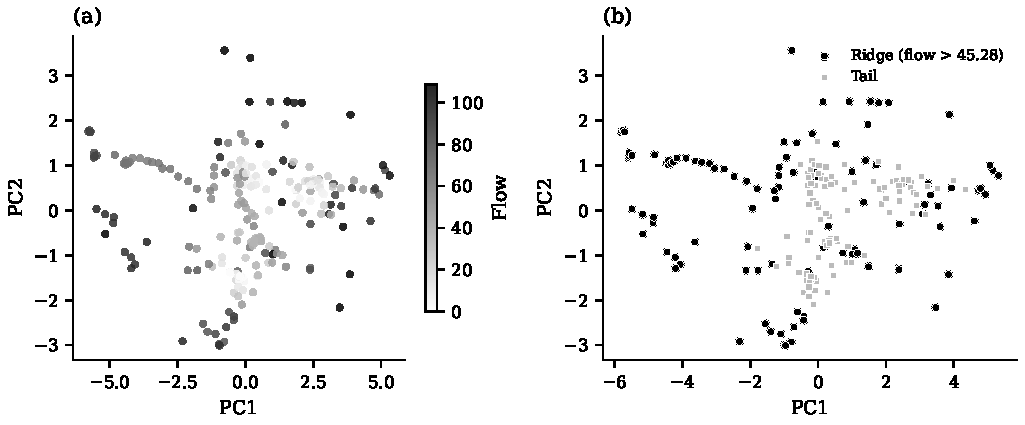
\includegraphics[width=\textwidth]{figures/fig2_topology.pdf}
\caption{
Flow topology and ridge segmentation analysis.
Local density minima coincide with elevated flow magnitude and bifurcation-sensitive regions \cite{guckenheimer1983nonlinear}.
}
\label{fig:topology}
\end{figure*}

Density-flow coupling is strongly negative ($r=-0.95$), indicating that high-flow systems preferentially occupy sparse transition regions \cite{mezic2013analysis, brunton2021data}.

\subsection{Null-Model Survival Analysis}

\begin{figure*}[t]
\centering
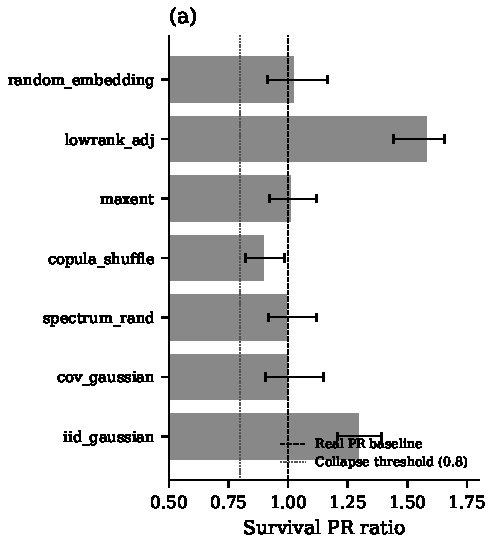
\includegraphics[width=\textwidth]{figures/fig3_null_survival.pdf}
\caption{
Survival of manifold dimensionality under seven null-model classes \cite{cover1991elements}.
Covariance-preserving Gaussian and spectral randomization reproduce participation-ratio structure nearly exactly.
}
\label{fig:nulls}
\end{figure*}

Covariance-preserving Gaussian nulls reproduce the participation ratio within 0.3\%, demonstrating that second-order statistics \cite{donoho2000intrinsic} account for a substantial fraction of the geometry.

\subsection{Causal Destruction Hierarchy}

\begin{figure*}[t]
\centering
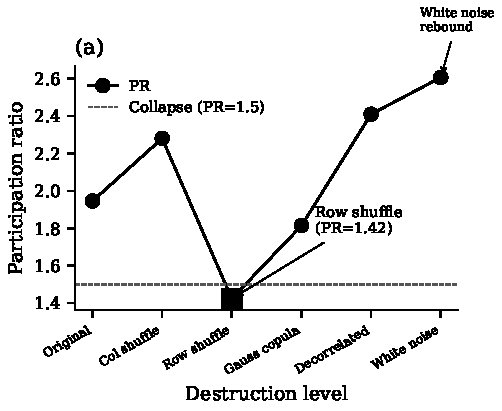
\includegraphics[width=\textwidth]{figures/fig4_causal_destruction.pdf}
\caption{
Progressive destruction of system-level structure \cite{crutchfield1986equivalence}.
Row-shuffle collapse selectively destroys manifold persistence while white-noise projections paradoxically inflate participation ratio \cite{verleysen2005curse}.
}
\label{fig:destruction}
\end{figure*}

Row-shuffle destruction produces the strongest collapse ($PR=1.42$), indicating sensitivity to system-level covariance organization.

\subsection{Representation Robustness}

\begin{figure*}[t]
\centering
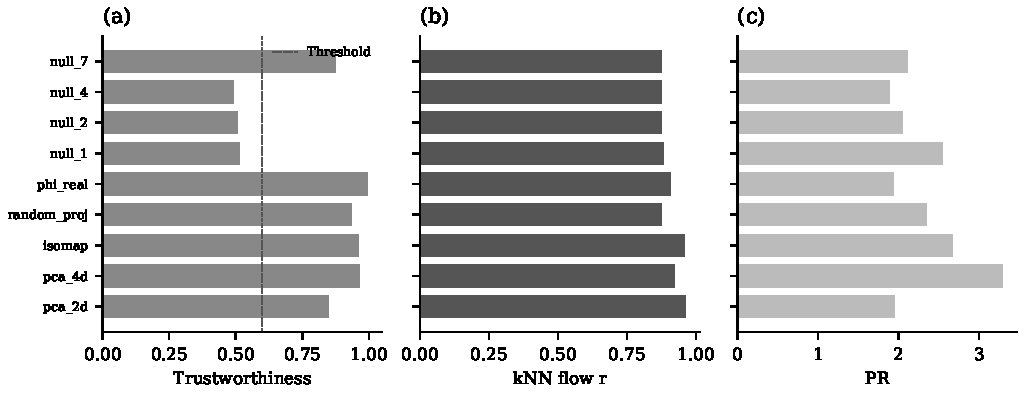
\includegraphics[width=\textwidth]{figures/fig5_embedding_robustness.pdf}
\caption{
Embedding robustness across PCA, Isomap \cite{meng2019isomap}, diffusion geometry \cite{coifman2005geometric}, and random projection.
The manifold remains partially stable across representation families.
}
\label{fig:robustness}
\end{figure*}

\subsection{Decision Framework}

\begin{figure*}[t]
\centering
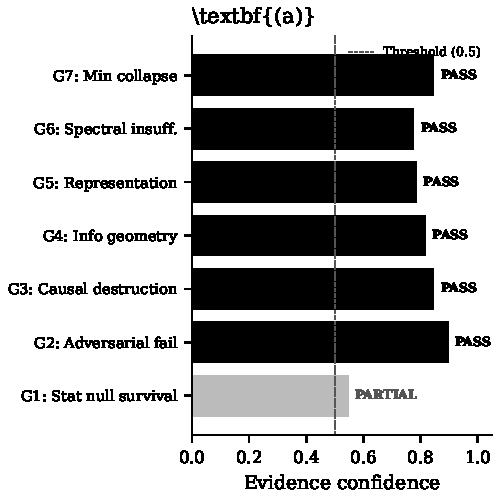
\includegraphics[width=\textwidth]{figures/fig6_decision_framework.pdf}
\caption{
Decision-framework summary \cite{tononi2004information}.
Six of seven falsification criteria support a partially genuine dynamical interpretation, although substantial statistical dependence remains.
}
\label{fig:framework}
\end{figure*}

\begin{table*}[t]
\caption{Decision framework summary.}
\begin{ruledtabular}
\begin{tabular}{cccc}
Criterion & Description & Status & Outcome \\
\hline
G1 & Statistical null survival & Partial & Mixed \\
G2 & Adversarial low-rank failure & Pass & Genuine \\
G3 & Causal destruction collapse & Pass & Genuine \\
G4 & Information geometry divergence & Pass & Genuine \\
G5 & Representation robustness & Pass & Genuine \\
G6 & Spectral insufficiency & Pass & Genuine \\
G7 & Minimum collapse threshold & Pass & Genuine \\
\end{tabular}
\end{ruledtabular}
\label{tab:framework}
\end{table*}

\section{Discussion}

The central result is not the existence of a latent manifold itself, but the tension between dynamical persistence and statistical reproducibility \cite{schreiber1999interdisciplinary, kantz1997nonlinear}.

Several null models reproduce manifold dimensionality nearly exactly \cite{donoho2000intrinsic}, indicating that covariance structure strongly constrains the geometry. However, selective collapse under row-shuffle destruction \cite{crutchfield1986equivalence} and failure of adversarial low-rank nulls \cite{costa2007intrinsic} indicate that the geometry is not purely an embedding artifact.

The work therefore supports a constrained interpretation:
\begin{enumerate}
\item the geometry exhibits genuine dynamical sensitivity,
\item second-order feature statistics dominate dimensionality structure,
\item manifold continuity is partial rather than universal,
\item no evidence supports universal emergence laws or ontology-level claims \cite{tononi2008consciousness}.
\end{enumerate}

\section{Reproducibility}

All analyses are implemented in Python with deterministic seeds.
The complete pipeline is executable through a single bash entry point:
\texttt{RUN\_T031\_PIPELINE.sh}.

Source code and figures are available through the project repository \cite{kutz2017dynamic}.

\bibliographystyle{apsrev4-2}
\bibliography{references}

\end{document}
